\documentclass[UTF8]{ctexart}
\usepackage{amsmath}
\usepackage{float}
\usepackage{indentfirst}
\usepackage{listings}
\usepackage{xcolor}
\lstset{
    %backgroundcolor=\color{red!50!green!50!blue!50},%代码块背景色为浅灰色
    rulesepcolor= \color{gray}, %代码块边框颜色
    breaklines=true,  %代码过长则换行
    numbers=left, %行号在左侧显示
    numberstyle= \small,%行号字体
    %keywordstyle= \color{red},%关键字颜色
    %commentstyle=\color{green!90}, %注释颜色
    frame=shadowbox%用方框框住代码块
    }
\usepackage{graphicx}
\usepackage[a4paper, left = 3.17cm, right = 3.17cm, top=2.54cm, bottom=2.54cm]{geometry}
\setlength{\parindent}{2em}
\title{第三讲-习题}
\author{姜帆}
\date{\today}
\begin{document}
\maketitle
\tableofcontents
\newpage
\section{LM算法}
\subsection{阻尼因子变化曲线图}
\begin{figure}[H]
\centering
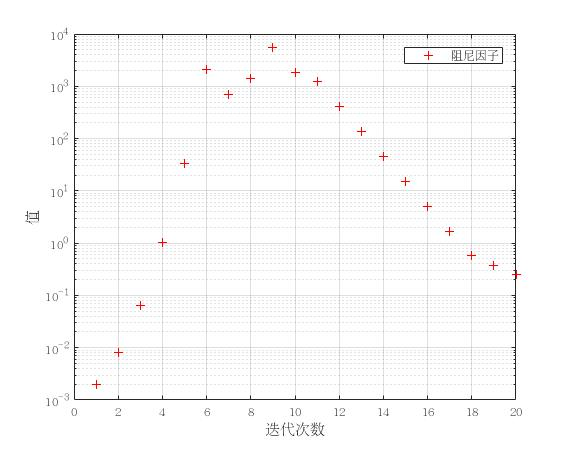
\includegraphics[width=0.9\textwidth]{mu1_g.jpg}    
\caption{阻尼因子变化曲线图}
\label{img0}
\end{figure}
\indent 下图为程序运行结果:\\
\begin{figure}[H]
\centering
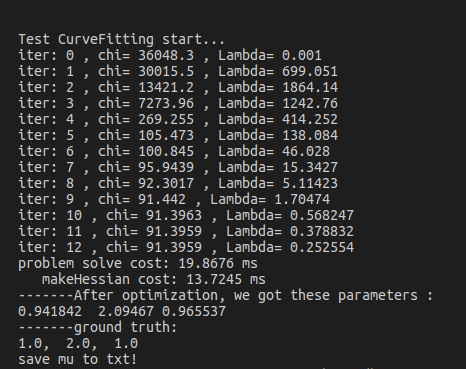
\includegraphics[width=0.8\textwidth]{mu1.jpg}    
\caption{程序运行结果}
\label{imga}
\end{figure}

\subsection{更改曲线函数}
\indent 将曲线函数改为$y=ax^2+bx+c$,修改对应雅克比计算函数,残差计算函数。另注意由于生成仿真数据时添加了均值为0,方差为1的噪声项,
噪声相对于数据较大,因此对增加仿真数据量。\\
\indent $y=ax^2+bx+c$函数对应的雅克比计算函数(导数)为$y'=x^2+x+1$
\begin{lstlisting}[language={c++}]
    class CurveFittingEdge: public Edge
    {
    public:
        EIGEN_MAKE_ALIGNED_OPERATOR_NEW
        CurveFittingEdge( double x, double y ): Edge(1,1, std::vector<std::string>{"abc"}) {
            x_ = x;
            y_ = y;
        }
        // 计算曲线模型误差
        virtual void ComputeResidual() override
        {
            Vec3 abc = verticies_[0]->Parameters();  // 估计的参数
            //residual_(0) = std::exp( abc(0)*x_*x_ + abc(1)*x_ + abc(2) ) - y_;  // 构建残差
            residual_(0) = abc(0)*x_*x_ + abc(1)*x_ + abc(2) - y_;  // 构建残差 
        }
    
        // 计算残差对变量的雅克比
        virtual void ComputeJacobians() override
        {
            Vec3 abc = verticies_[0]->Parameters();
            double exp_y = std::exp( abc(0)*x_*x_ + abc(1)*x_ + abc(2) );
    
            Eigen::Matrix<double, 1, 3> jaco_abc;  // 误差为1维,状态量 3 个,所以是 1x3 的雅克比矩阵
            //jaco_abc << x_ * x_ * exp_y, x_ * exp_y , 1 * exp_y;
            jaco_abc << x_ * x_ , x_ , 1;
            jacobians_[0] = jaco_abc;
        }
        /// 返回边的类型信息
        virtual std::string TypeInfo() const override { return "CurveFittingEdge"; }
    public:
        double x_,y_;  // x 值, y 值为 _measurement
    };  
\end{lstlisting}
\begin{figure}[H]
\centering
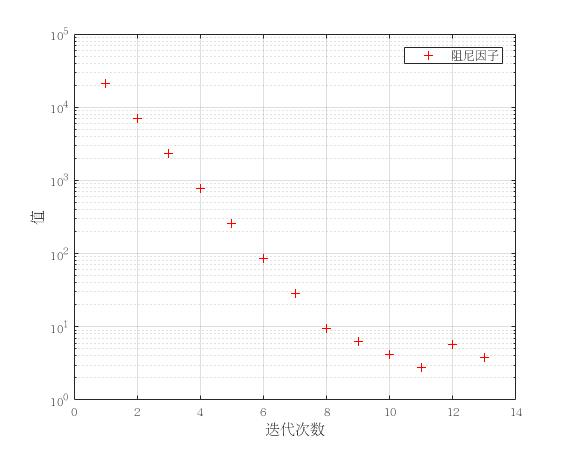
\includegraphics[width=0.9\textwidth]{mu2_g.jpg}    
\caption{阻尼因子变化曲线图}
\label{img1}
\end{figure}

\subsection{Marquardt阻尼因子更新策略}
\indent Marquardt阻尼因子更新策略如下:
\begin{equation}\nonumber
\begin{aligned}
    if \rho < 0.25 \\
    \mu := \mu*2\\
    if \rho > 0.75\\
    \mu :=\mu/3
\end{aligned}
\end{equation}
\indent 具体阻尼因子更新策略实现代码为:
\begin{lstlisting}[language={c++}]
    if(rho >= 0 && isfinite(tempChi))
    {
        if(rho < 0.25 )
            currentLambda_*=2;
        else if(rho >0.75)
            currentLambda_=currentLambda_/3;

        currentChi_ = tempChi;
        return true;
    }
    else 
    {
      currentLambda_ =currentLambda_ *2;
      return false;   
    }
\end{lstlisting}
\indent 下图为程序运行结果:\\
\begin{figure}[H]
\centering
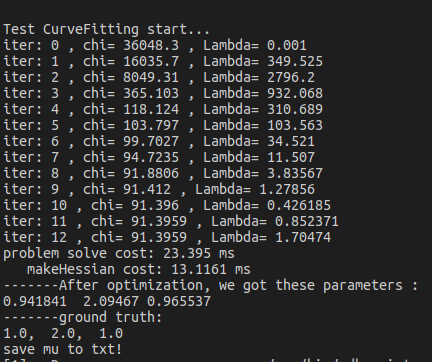
\includegraphics[width=0.8\textwidth]{mu2.jpg}    
\caption{程序运行结果}
\label{imga}
\end{figure}

\section{公式推导}
\subsection{$f_{15}$}
\indent $f_{15}$求的是位移预积分量对$k$时刻角速度$b_k^g$的Jacobian。\\
\indent 预积分的离散形式,其中积分方法采用中值积分,即两个相邻时刻$k$到$k+1$的位姿是用两个时刻的测量值的平均值来计算。
其中位移的预积分量为:\\
\begin{equation}
\begin{aligned}
&\alpha_{b_ib_{k+1}}=\alpha_{b_ib_k}+\beta_{b_ib_k}\delta t+\frac{1}{2}a \delta t^2\\
&a=\frac{1}{2}(q_{b_ib_k}(a^{b_k}-b_k^a)+q_{b_ib_{k+1}}(a^{b_{k+1}}-b_k^a))\\
&\omega=\frac{1}{2}((\omega^{b_k}-b_k^g)+(\omega^{b_{k+1}}-b_k^g))=\frac{1}{2}(\omega^{b_k}+\omega^{b_{k+1}})-b_k^g
\end{aligned}
\end{equation}
\indent 因此位移预积分量也可以写为:\\
\begin{equation}
\begin{aligned}
&\alpha_{b_ib_{k+1}}=\alpha_{b_ib_k}+\beta_{b_ib_k}\delta t+\frac{1}{2}a \delta t^2\\
&=\alpha_{b_ib_k}+\beta_{b_ib_k}\delta t+\frac{1}{4}(q_{b_ib_k}(a^{b_k}-b_k^a)+q_{b_ib_{k+1}}(a^{b_{k+1}}-b_k^a))\delta t^2\\
&=\alpha_{b_ib_k}+\beta_{b_ib_k}\delta t+\frac{1}{4}(q_{b_ib_k}(a^{b_k}-b_k^a)+q_{b_ib_k}\otimes
\left[\begin{array}{cccc} 
1 \\
\frac{1}{2}\omega\delta t
\end{array}\right] (a^{b_{k+1}}-b_k^a))\delta t^2\\
\end{aligned}
\end{equation}
\indent 其中只有括号加号后面一项与角速度$b_k^g$有关,因此$f_{15}$可以变为:\\
\begin{equation}
\begin{aligned}
&f_{15}=\frac{\partial\alpha _{b_ib_{k+1}}}{\partial\delta b_k^g}\\
&=\frac{1}{4}
\frac{ 
    \partial q_{b_ib_k}\otimes 
    \begin{bmatrix}
        1\\
        \frac{1}{2}\omega\delta t
    \end{bmatrix}
    \otimes
    \begin{bmatrix}
        1\\
        -\frac{1}{2}\delta b_k^g \delta t
    \end{bmatrix}  (a^{b_{k+1}}-b^a_k)\delta t^2
}{\partial \delta b_k^g}\\
&=\frac{1}{4}\frac
{
    \partial R_{b_1b_{k+1}}exp([-\delta b_k^g \delta t]_\times)
    (a^{b_{k+1}}-b^a_k)\delta t^2
}
{\partial \delta b_k^g}\\
&=\frac{1}{4}\frac
{
    \partial R_{b_1b_{k+1}}(I+[-\delta b_k^g \delta t]_\times)
    (a^{b_{k+1}}-b^a_k)\delta t^2 
}{\partial \delta b_k^g}\\
&=\frac{1}{4}\frac
{
    \partial R_{b_1b_{k+1}}[-\delta b_k^g \delta t]_\times
    (a^{b_{k+1}}-b^a_k)\delta t^2 
}{\partial \delta b_k^g}\\
&=-\frac{1}{4}\frac
{
    \partial R_{b_1b_{k+1}}[(a^{b_{k+1}}-b^a_k)]_\times \delta t^2
    (-\delta b_k^g \delta t)   
}{\partial \delta b_k^g}\\
&=-\frac{1}{4} R_{b_1b_{k+1}}[(a^{b_{k+1}}-b^a_k)]_\times \delta t^2(- \delta t)\\
\end{aligned}
\end{equation}

\subsection{${g_{12}}$}
\indent $f_{15}$求的是位移预积分量对$k$时刻角速度的噪声$n_{b_k^g}$的Jacobian。\\
\indent 将角速度测量噪声也考虑进模型,预积分的离散形式,其中积分方法采用中值积分,即两个相邻时刻$k$到$k+1$的位姿是用两个时刻的测量值的平均值来计算。
其中位移的预积分量为:\\
\begin{equation}
\begin{aligned}
&\alpha_{b_ib_{k+1}}=\alpha_{b_ib_k}+\beta_{b_ib_k}\delta t+\frac{1}{2}a \delta t^2\\
&a=\frac{1}{2}(q_{b_ib_k}(a^{b_k}-b_k^a)+q_{b_ib_{k+1}}(a^{b_{k+1}}-b_k^a))\\
&\omega=\frac{1}{2}((\omega^{b_k}+n_k^g-b_k^g)+(\omega^{b_{k+1}}+n_{k+1}^g-b_k^g))=\frac{1}{2}(\omega^{b_k}+n_k^g+\omega^{b_{k+1}}+n_{k+1}^g)-b_k^g
\end{aligned}
\end{equation}
\indent 因此位移预积分量也可以写为:\\
\begin{equation}
\begin{aligned}
&\alpha_{b_ib_{k+1}}=\alpha_{b_ib_k}+\beta_{b_ib_k}\delta t+\frac{1}{2}a \delta t^2\\
&=\alpha_{b_ib_k}+\beta_{b_ib_k}\delta t+\frac{1}{4}(q_{b_ib_k}(a^{b_k}-b_k^a)+q_{b_ib_{k+1}}(a^{b_{k+1}}-b_k^a))\delta t^2\\
&=\alpha_{b_ib_k}+\beta_{b_ib_k}\delta t+\frac{1}{4}(q_{b_ib_k}(a^{b_k}-b_k^a)+q_{b_ib_k}\otimes
\left[\begin{array}{cccc} 
1 \\
\frac{1}{2}\omega\delta t
\end{array}\right] (a^{b_{k+1}}-b_k^a))\delta t^2
\end{aligned}
\end{equation}
\indent 其中只有括号加号后面一项与角速度的噪声$n_{b_k^g}$有关,因此$g_{12}$可以变为:\\
\begin{equation}
\begin{aligned}
&g_{12}=\frac{\partial \alpha_{b_ib_k}}{\partial n_{b_k^g}}\\
&=\frac{1}{4}\frac
{
    \partial q_{b_ib_k}\otimes 
    \begin{bmatrix}
        1\\
        \frac{1}{2}\omega\delta t
    \end{bmatrix}
    \otimes
    \begin{bmatrix}
        1\\
        \frac{1}{4}\delta n_{b_k^g} \delta t
    \end{bmatrix}  (a^{b_{k+1}}-b^a_k)\delta t^2
}{\partial n_{b_k^g}}\\
&=\frac{1}{4}\frac
{
    \partial R_{b_1b_{k+1}}exp([\frac{1}{2}\delta n_{b_k^g} \delta t]_\times)
    (a^{b_{k+1}}-b^a_k)\delta t^2 
}{\partial n_{b_k^g}}\\
&=\frac{1}{4}\frac
{
    \partial R_{b_1b_{k+1}}(I+[\frac{1}{2}\delta n_{b_k^g} \delta t]_\times)
    (a^{b_{k+1}}-b^a_k)\delta t^2 
}{\partial n_{b_k^g}}\\
&=\frac{1}{4}\frac
{
    \partial R_{b_1b_{k+1}}[\frac{1}{2}\delta n_{b_k^g} \delta t]_\times
    (a^{b_{k+1}}-b^a_k)\delta t^2 
}{\partial n_{b_k^g}}\\
&=-\frac{1}{4}\frac
{
    \partial R_{b_1b_{k+1}}[(a^{b_{k+1}}-b^a_k)]_\times(\frac{1}{2}\delta n_{b_k^g} \delta t)\delta t^2 
}{\partial n_{b_k^g}}\\
&=-\frac{1}{4}R_{b_1b_{k+1}}[(a^{b_{k+1}}-b^a_k)]_\times(\frac{1}{2} \delta t)\delta t^2 \\
\end{aligned}
\end{equation}

\section{证明}
\indent L-M优化算法中,引入阻尼因子,如下式:\\
\begin{equation}
\begin{aligned}
& (J^TJ+\mu I) \Delta x_{lm}=-J^Tf
\end{aligned}
\end{equation}
\indent 半正定的信息矩阵$J^tJ$特征值${\lambda_j}$和对应的特征向量为${v_j}$。对$J^TJ$做特征值分解分解后有:
$J^TJ=V\Lambda V^T$。\\
\indent $J^TJ$为对称矩阵,对对称矩阵做特征值分解有$J^TJ=V\Lambda V^T$,其中$V^TV=VV^T=I$。\\
\indent 有$F'=(J^Tf)^T$。\\
\indent 证明:\\
\indent 根据$J^TJ=V\Lambda V^T$和$VV^T=I$,$(J^TJ+\mu I)\Delta x_{lm}=-J^T$可以写为:
\begin{equation}
\begin{aligned}
&(V\Lambda V^T+\mu I)\Delta x_{lm} = - F'^T\\
&(V(\Lambda+\mu I)V^T)\Delta x_{lm} = - F'^T\\
\end{aligned}
\end{equation}
\indent 等式两边同时左乘 $V^T$,右乘$V$,则有:
\begin{equation}
\begin{aligned}
&(\Lambda+\mu I)\Delta x_{lm} = - V^TF'^TV\\
&\Delta x_{lm}=-\frac{V^TF'^TV}{\Lambda+\mu I}
\end{aligned}
\end{equation}
\indent 其中:\\
\begin{equation}
V=
\begin{bmatrix}
v_1 & v_2 & ... & v_n
\end{bmatrix}^T
\end{equation}
\begin{equation}
%\begin{aligned}
\Lambda=
\begin{bmatrix}
\lambda_1\\
&\lambda_2 & & \text{{\huge 0}}\\
&&\dots\\
& \text{{\huge 0}} && \lambda_{n-1}\\
&&&& \lambda_n
\end{bmatrix}
%\end{aligned}
\end{equation}

\begin{equation}
%\begin{aligned}
\mu I=
\begin{bmatrix}
    \mu\\
&\mu& & \text{{\huge 0}}\\
&&\dots\\
& \text{{\huge 0}} && \mu\\
&&&& \mu
\end{bmatrix}
%\end{aligned}
\end{equation}
\indent 因此变为:\\
\begin{equation}
\begin{aligned}
&\Delta x_{lm}=-\frac
{
    \begin{bmatrix}
    v_1 & v_2 & ... & v_n
    \end{bmatrix}F'^T
    \begin{bmatrix}
    v_1 \\ v_2 \\ ... \\ v_n
    \end{bmatrix}
}
{
    \begin{bmatrix}
    \lambda_1\\
    &\lambda_2 & & \text{{\huge 0}}\\
    &&\dots\\
    & \text{{\huge 0}} && \lambda_{n-1}\\
    &&&& \lambda_n
    \end{bmatrix}
    +
    \begin{bmatrix}
        \mu\\
    &\mu& & \text{{\huge 0}}\\
    &&\dots\\
    & \text{{\huge 0}} && \mu\\
    &&&& \mu
    \end{bmatrix}
}\\
&=-\sum_{i=1}^n\frac{v_j^TF'^Tv_j}{\lambda _j + \mu}
\end{aligned}
\end{equation}

\end{document}